\documentclass[11pt,a4paper,fontset=macnew]{ctexart}
\usepackage[top=2.5cm,bottom=2.5cm,left=3cm,right=3cm]{geometry}
\usepackage{amsmath,amssymb}
\usepackage{booktabs}
\usepackage{array}
\usepackage{longtable}
\usepackage{graphicx}
\usepackage{caption}
\usepackage{hyperref}
\usepackage{xcolor}
\usepackage{fancyhdr}
\usepackage{titlesec}
\usepackage{tikz}
\usepackage{float}

\hypersetup{
  colorlinks=true,
  linkcolor=blue,
  urlcolor=blue,
  citecolor=blue
}

\captionsetup{font=small,labelfont=bf}
\graphicspath{{figures/}}

\pagestyle{fancy}
\fancyhf{}
\fancyhead[L]{\small 2026 中国研究生人工智能创新大赛 · 华为赛题三}
\fancyhead[R]{\small 智能论文搜索系统 eZScholar 项目提案}
\fancyfoot[C]{\thepage}

\titleformat{\section}{\Large\bfseries}{\thesection}{1em}{}
\titleformat{\subsection}{\large\bfseries}{\thesubsection}{1em}{}
\titleformat{\subsubsection}{\normalsize\bfseries}{\thesubsubsection}{1em}{}

\newcommand{\placeholder}[1]{%
  \begin{center}
  \fbox{\parbox{0.85\textwidth}{\centering\vspace{0.6cm}
  \textbf{[ 插图预留位 ]}\\[0.2cm]
  #1\vspace{0.6cm}}}
  \end{center}
}

\title{\vspace{-1.5em}\textbf{\Large 科研场景下复杂学术查询的智能论文搜索与推荐系统}\\[0.4em]
\large —— eZScholar 智能学术检索 Agent\\[0.3em]
\large 项目提案与实施方案（技术方案分册）}
\author{\large 参赛团队}
\date{\large 2026 年 8 月}

\begin{document}

\maketitle
\thispagestyle{fancy}

\tableofcontents
\newpage

% =========================================================
\section{项目概况}
\label{sec:overview}

\subsection{项目背景与问题定义}
\label{sec:background}

本项目参加 2026 年中国研究生人工智能创新大赛（华为赛题三《科研场景下复杂学术查询的智能论文搜索与推荐》）。赛题要求参赛队伍构建能够理解复杂学术查询、自主完成多轮检索、输出结构化高质量结果的智能论文搜索与推荐系统。评测综合考察检索质量（F1，占 70\%）、运行效率（占 20\%）与结构化输出（占 10\%）三个维度，既考核算法的检索精度，也考核系统的工程能力与可复现性。

在科研活动中，文献检索是最基础也是最耗时的工作之一。研究人员面对的是一个规模庞大且仍在快速增长的全球知识网络：以开放学术目录 OpenAlex 为例，其已收录超过 2.4 亿篇学术成果，涵盖期刊论文、专著、数据集、学位论文与预印本，并依托 Crossref、ORCID、ROR 等权威来源每日增量更新。信息过载与检索工具能力不足之间的矛盾日益突出，"找得全、找得准、找得快"已成为科研用户的刚性需求。

传统学术搜索引擎（如 Google Scholar、Semantic Scholar）对\textbf{短查询、关键词式查询}表现良好，但对\textbf{复杂学术查询}——即由多个研究侧面、限定条件与隐性约束构成的自然语言长句——召回质量显著下降。经过对真实科研查询的分析，这类复杂查询普遍具备以下特征：

\begin{itemize}
  \item \textbf{语义复合}：一个查询同时包含研究对象、研究方法、应用场景、对比基线等多个维度，难以用单一关键词覆盖；
  \item \textbf{术语漂移}：查询使用的口语化词汇与目标论文标题、摘要中的学术术语重叠度低，直接检索命中困难；
  \item \textbf{隐含约束}：用户往往隐含"该领域代表性工作""近三年""与某方法形成对比"等未明确说出的要求；
  \item \textbf{结果组织}：用户不仅需要论文列表，更期望获得按主题组织的结构化归纳与可解释的证据支撑。
\end{itemize}

2025 年，字节跳动研究团队在 ACL 2025 发表的 \emph{PaSa}（\cite{pasa2025}）正式提出这一挑战，并构建了面向真实场景的基准数据集 \textbf{RealScholarQuery}——由 50 条 AI 研究者真实提出的细粒度科研查询构成，答案由专业标注员逐一确认。实验结果显示，即便是 GPT-4o 配合 Google 检索改写的强基线，在 RealScholarQuery 上的 Recall@20 也比专门训练的 PaSa-7B 检索 Agent 低 37.78\%。这一结果表明：\textbf{复杂学术查询的检索问题并未被通用工具解决，亟需专门的检索智能体}，而这正是本项目的切入点。

\subsection{已有基础与研究积累}
\label{sec:foundation}

本项目并非从零起步。团队此前完成了可迁移的工程可信智能体架构 eZmanbo（电子元器件智能选型与风险评估 Agent），并将其验证过的核心机制——统一中间表示、约束解析、多路召回、评分门禁、硬约束校验、证据链、工具编排、缓存降级——迁移改造为学术检索 Agent \textbf{eZScholar}（项目代号 ScholarTrace），已在真实服务器完成原型开发与多轮评测：

\begin{itemize}
  \item \textbf{统一核心对象}：QueryIR（查询中间表示）、SubQuery（子查询）、PaperIdentity（论文身份）、PaperEvidence（证据链）、SearchTrace（执行轨迹）、RankResult（排序结果）、RunReport（运行报告），所有环节以结构化对象流转；
  \item \textbf{先宽后窄两阶段 Agent 流程}：Round0 查询解析 → Round1 宽召回 → Round2 引文扩展 → Round3 精排清理 → 早停决策；
  \item \textbf{免 Key 学术 API 适配}：OpenAlex 主召回、Crossref 身份对齐、Semantic Scholar 引文推荐、Unpaywall 开放获取、arXiv 预印本、OpenCitations 引文图；
  \item \textbf{完整评测阶梯}：B0（词法基线）→ B1（查询理解+子查询）→ B2（引文扩展）→ B3（LLM 精排）→ B4（缓存+预算早停）→ FULL 全链路，统一评测框架；
  \item \textbf{评测数据对齐}：基于 PaSa RealScholarQuery 基准，gold 论文按 OpenAlex ID / DOI / 归一化标题三重匹配对齐，避免同一论文多条记录导致的虚增。
\end{itemize}

截至本提案撰写时，系统已完成 50 条 RealScholarQuery 全量离线评测（OpenAlex 口径）：\textbf{平均 F1 = 0.0774，召回率 R = 0.0950，精确率 P = 0.1042}；其中 26 条查询 F1 > 0，16 条 F1 $\geq$ 0.1，最高单条 F1 = 0.370。与 B0 词法基线（平均 F1 = 0.0095）相比提升超过 8 倍，验证了"查询理解 + 子查询分解"作为第一技术杠杆的路线正确性。

\subsection{项目目标与价值}
\label{sec:goals}

本项目的总体目标是：\textbf{构建一个面向科研场景的复杂学术查询智能搜索与推荐系统}，通过"查询理解 → 查询规划 → 多路召回 → 质量门禁 → 综合精排 → 迭代搜索 → 证据输出 → 预算控制"的完整链路，将复杂自然语言查询转化为高质量、可溯源、结构化的学术论文检索结果，并满足比赛对\textbf{检索质量（F1）、运行效率、结构化输出}三方面权重的综合要求。

\begin{table}[H]
\centering
\caption{比赛评测权重构成与项目应对策略}
\label{tab:weights}
\small
\begin{tabular}{@{}lcc@{}}
\toprule
\textbf{评测维度} & \textbf{权重} & \textbf{项目应对} \\
\midrule
检索质量（F1） & 70\% & 查询理解 + 子查询分解 + LLM 精排 + 引文扩展 \\
运行效率 & 20\% & 缓存复用、预算早停、分层 LLM Router、并发限流 \\
结构化输出 & 10\% & 统一 Schema、证据链、结构化归纳展示 \\
\bottomrule
\end{tabular}
\end{table}

项目价值体现在三个层面：

\begin{enumerate}
  \item \textbf{对科研用户}：显著降低文献调研成本，将"检索"从关键词匹配升级为"研究问题的结构化求解"，让研究者把时间投入到真正的科研创造上；
  \item \textbf{对比赛评测}：以冻结数据、可复现评测、可审计轨迹满足竞赛对公平性与可信性的硬性要求，评测口径全程透明可追溯；
  \item \textbf{对技术体系}：沉淀一套可迁移的"领域知识获取 + 智能体工具编排 + 预算控制"工程范式，未来可复用到智能问答、知识服务等多个方向。
\end{enumerate}

\subsection{场景分析与应用前景}
\label{sec:scenario}

从应用场景看，复杂学术查询搜索系统至少可服务于三类用户：

\begin{itemize}
  \item \textbf{科研新手}：面对陌生研究方向时，需要"研究问题 → 代表工作 → 方法谱系"的引导式检索，帮助快速建立领域地图；
  \item \textbf{资深研究者}：需要针对具体方法做系统性调研与对比，关注方法演进的引用链条与相关工作边界；
  \item \textbf{科研管理人员}：需要按主题聚合文献并生成结构化概览，用于学科布局、方向评估与决策支持。
\end{itemize}

三种场景对"检索质量 + 结构化归纳 + 可解释证据"的需求是共通的，这进一步支撑了本项目的技术路线选择。

结合本赛题（华为赛题三《科研场景下复杂学术查询的智能论文搜索与推荐》）的考核要点，本项目的功能点映射关系如下：

\begin{itemize}
  \item \textbf{查询理解与分解}：对应 Round0 查询解析与子查询规划，将复杂长句拆解为可执行的检索单元；
  \item \textbf{自主检索迭代}：对应 Round1 多路召回与 Round2 引文扩展，系统可在无人干预下自主完成多轮检索；
  \item \textbf{综合排序}：对应 Round3 LLM 精排，综合语义相关度、证据强度与约束满足度给出最终排序；
  \item \textbf{结构化展示与归纳}：对应证据输出层的查询摘要、论文分组与总体结论，输出可直接用于文献综述；
  \item \textbf{对接学术数据库}：对应 OpenAlex / Crossref / S2 等免 Key 学术 API 的适配层；
  \item \textbf{成本控制}：对应预算早停与缓存复用机制，保证系统在有限资源下稳定运行。
\end{itemize}

\subsection{资源需求}
\label{sec:resources}

项目运行不依赖自建大规模论文全文库，主要资源由学术检索接口、大语言模型推理接口、常规计算环境、缓存存储与稳定网络组成，资源需求如下：

\begin{table}[H]
\centering
\caption{资源需求与用途}
\label{tab:resources}
\small
\begin{tabular}{@{}lll@{}}
\toprule
\textbf{支持类别} & \textbf{主要内容} & \textbf{用途} \\
\midrule
学术数据接口 & OpenAlex 等开放学术检索接口 & 论文召回、论文身份及基础元数据获取 \\
模型推理能力 & 大语言模型 API（DeepSeek） & 复杂问题理解、查询规划、候选语义判断 \\
计算与存储 & 常规 CPU 服务器或个人计算机、实验缓存空间 & 运行检索流程、保存响应缓存与评测产物 \\
开发环境 & Python 运行环境及版本管理工具 & 系统开发、自动评测与实验复现 \\
网络环境 & 稳定的外部 API 访问能力 & 在线学术检索和模型调用 \\
\bottomrule
\end{tabular}
\end{table}

% =========================================================
\section{项目规划}
\label{sec:plan}

\subsection{总体技术路线}
\label{sec:roadmap}

项目采用\textbf{以查询理解为第一杠杆、以多路召回为覆盖基础、以 LLM 精排为质量核心、以预算控制为工程约束}的四层技术路线，构成"先宽后窄"的检索闭环：

\begin{enumerate}
  \item \textbf{Round0 查询解析}：将复杂自然语言查询解析为结构化 QueryIR（研究主题、方法、应用、约束、年限等字段），再由规划器生成多个子查询；
  \item \textbf{Round1 宽召回}：对规划子查询执行多路召回（OpenAlex 主召回 + 联想词专名召回 + 免 Key API 补充），最大化候选池覆盖；
  \item \textbf{Round2 引文扩展}：基于种子论文的引用与被引关系沿引文图扩展（Semantic Scholar 或 OpenCitations），捕获主题接近但词面不重叠的工作；
  \item \textbf{Round3 精排清理}：LLM 综合精排，输出 score / label / reason 与证据链，动态截断并过滤不相关候选；
  \item \textbf{早停与预算控制}：依据预算上限（API 调用数、token 数）与高相关收敛信号决定是否提前终止，控制运行成本。
\end{enumerate}

\begin{figure}[H]
\centering
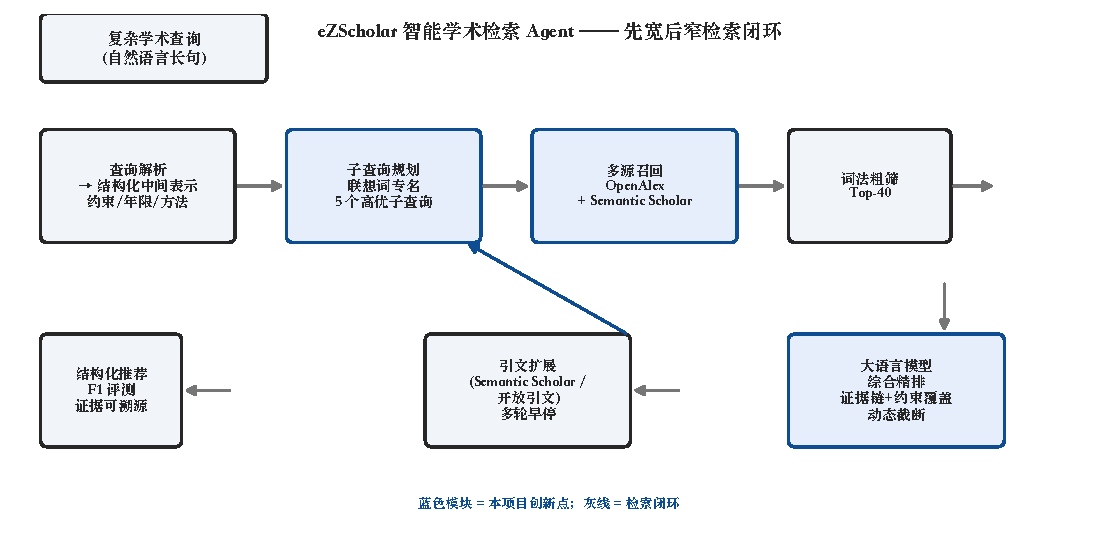
\includegraphics[width=0.95\textwidth]{fig1_pipeline}
\caption{eZScholar 系统架构与"先宽后窄"检索闭环。查询经结构化解析后生成多个子查询与联想词专名子查询（创新点 1），依次执行多源召回、词法粗筛、引文扩展与大语言模型（LLM）综合精排，最终输出带证据链的结构化推荐。蓝色模块为本项目创新点；LLM 指大语言模型，OpenAlex 与 Semantic Scholar 为两个主流开放学术文献数据源。}
\label{fig:pipeline}
\end{figure}

\begin{table}[H]
\centering
\caption{B0–FULL 实验阶梯与功能点对齐}
\label{tab:ladder}
\small
\begin{tabular}{@{}lll@{}}
\toprule
\textbf{实验阶梯} & \textbf{功能定位} & \textbf{对齐赛题功能点} \\
\midrule
B0 词法基线 & 直接查询 OpenAlex + 词法排序 & 检索能力（下限对照） \\
B1 查询理解 & QueryIR + 子查询分解 + 联想词 & 查询理解 / 分解 \\
B2 引文扩展 & S2 / OpenCitations 引文图 & 自主检索迭代 \\
B3 LLM 精排 & 综合相关度 + 证据链 & 综合排序 \\
B4 缓存预算 & 磁盘缓存 + 预算早停 & 成本控制 \\
FULL 全链路 & 多轮扩展 + 早停决策 + 归纳 & 结构化展示 / 全功能点 \\
\bottomrule
\end{tabular}
\end{table}

\begin{table}[H]
\centering
\caption{FAST 与 DEEP 双模式定位}
\label{tab:modes}
\small
\begin{tabular}{@{}llp{7.5cm}@{}}
\toprule
\textbf{模式} & \textbf{主要流程} & \textbf{定位} \\
\midrule
FAST & Round-1 查询规划 $\rightarrow$ OpenAlex 召回 $\rightarrow$ 去重与候选池 $\rightarrow$ LLM 精排 $\rightarrow$ 结构化输出 & 默认竞赛评测模式，优先保证效率与稳定性 \\
DEEP & FAST + Round-1 Observation $\rightarrow$ 二轮 Planner $\rightarrow$ Follow-up 检索 $\rightarrow$ Merge $\rightarrow$ 精排 & 复杂问题的可选深度检索与 Agentic Search 展示模式 \\
\bottomrule
\end{tabular}
\end{table}

\subsection{项目里程碑}
\label{sec:milestone}

依据比赛时间窗（报名 8 月 25 日截止、赛题提交 9 月 11 日），项目划分为三个阶段：

\begin{itemize}
  \item \textbf{第一阶段——基线验证（已完成）}：完成仓库搭建、B0 词法基线评测、核心数据结构定义、评测框架构建、挑战查询整理；
  \item \textbf{第二阶段——能力建设（已完成）}：完成查询理解、多路召回、引文扩展、LLM 精排、全链路集成与 50 条基准全量评测；
  \item \textbf{第三阶段——冻结与交付（进行中）}：冻结评测数据集、对齐 gold 身份、FULL 冻结验证、复现包构建、前端页面开发与答辩准备。
\end{itemize}

\subsection{技术创新点}
\label{sec:innovation}

\textbf{创新点 1：联想词专名召回机制。}针对"查询词汇与论文标题零重叠"这一核心召回失败根因（实测占 184 篇真值论文未命中的 88\%），本系统在规划阶段要求大语言模型（LLM）提炼代表性论文标题关键词（联想词），以独立高优先级子查询执行。实测该查询公式化策略使独立真值论文召回量由基线 22 篇提升至 25 篇（+3），配合提示词优化进一步增至 26 篇；叠加 Semantic Scholar 多源召回后，在 OpenAlex 之上额外新增 13 篇真值论文（+7.1\%）。离线消融进一步表明，关闭联想词候选的保送机制（assoc safepass）不改变原始召回，却使进入精排池的独立真值论文由 24 降至 13、最终独立真值论文由 16 降至 11、平均 F1 由 0.0618 降至 0.0485——该机制的作用不是制造更多召回，而是保护联想词已发现的候选不被词法粗筛提前丢弃。该机制以轻量方式复现了 PaSa 中"LLM 先验回忆"的关键作用，且不依赖复杂的强化学习训练。

\begin{table}[H]
\centering
\caption{查询公式化与迭代检索的召回增益（真值论文数为去重后的独立命中数；真值论文即基准中人工标注的正确论文）}
\label{tab:formulation}
\small
\begin{tabular}{@{}llcc@{}}
\toprule
\textbf{优化环节} & \textbf{策略} & \textbf{独立真值论文数} & \textbf{增量} \\
\midrule
查询公式化 & 初始基线 & 22 & --- \\
 & 追加联想词子查询 & 25 & +3 \\
 & 提示词优化 & 26 & +1 \\
\midrule
证据引导迭代检索 & 单轮检索 & 25 & --- \\
 & 合并多轮检索 & 27 & +2（2/22 查询） \\
\bottomrule
\end{tabular}
\end{table}

\textbf{创新点 2：统一中间表示与可审计执行轨迹。}所有检索环节以 QueryIR / SubQuery / PaperIdentity / SearchTrace 等结构化对象流转，全程落盘可追溯，兼顾评测可复现性与证据链可解释性，为后续的失败归因与迭代优化提供了完整的观测基础。

\textbf{创新点 3：基于边际检索收益的预算重分配。}磁盘召回缓存跨实验复用、计划缓存（query → IR + 子查询）避免非确定性重复消耗、预算与 token 双层早停、LLM 失败自动降级，构建了可上线、成本可控的检索系统。在此基础上，阶段级追踪对每个检索阶段记录逻辑 API 调用、候选增量与目标论文命中，量化各阶段\textbf{边际收益}：受控实验中，无差别执行引文、参考与元数据扩展合计消耗 422 次逻辑调用却未带来任何新增命中，关闭后单查询逻辑调用由 511 降至 87，平均 F1 反而由 0.0528 提升至 0.0618（表 \ref{tab:budget}）。系统据此将预算优先配置给直接检索与高价值查询规划，实现"低成本不损质量"的预算重分配，契合比赛对运行效率的考核。

\textbf{创新点 4：双源引文扩展。}有 Semantic Scholar Key 时走 Semantic Scholar（S2）引文链，无 Key 时自动切换 OpenCitations（COCI，无 Key 引文图），保证引文扩展在任何环境下均可运行，提升了系统的环境适应性与鲁棒性。

\subsection{与现有工作的差异化}
\label{sec:difference}

与 PaSa（\cite{pasa2025}）等代表性工作相比，本项目在以下三方面形成差异化：

\begin{itemize}
  \item \textbf{轻量化与低成本}：PaSa 需要大规模合成数据训练与强化学习优化，而本系统采用免训练的提示工程方案，仅依赖通用 LLM API 与免 Key 学术数据源即可运行，更契合比赛对运行效率的约束；
  \item \textbf{强可审计性}：本系统以统一中间表示与 SearchTrace 轨迹记录每一次检索、扩展与精排决策，支持逐条失败归因，而 PaSa 类方法更侧重端到端效果，内部决策可解释性较弱；
  \item \textbf{工程可信优先}：本系统将缓存复用、预算早停、降级容错作为一等公民设计，保证在有限配额、网络抖动、模型不可用等现实约束下仍能产出稳定结果。
\end{itemize}

这种差异化定位使本项目在"检索效果 + 工程可信 + 成本可控"三个维度上取得平衡，符合赛事对综合性工程能力的要求。

% =========================================================
\section{实施方案}
\label{sec:impl}

\subsection{系统总体架构}
\label{sec:architecture}

系统总体架构如图所示（前端页面正在开发，插图位置预留）：

\placeholder{图 1：eZScholar 系统总体架构图（查询理解 → 查询规划 → 多路召回 → PaperIR → 质量门禁 → 精排 → 迭代搜索 → 证据输出 → 预算控制）。前端页面开发完成后替换为正式架构图。}

系统由以下分层构成：

\begin{enumerate}
  \item \textbf{接入层}：FastAPI 提供 \texttt{/search} 搜索接口与 \texttt{/health} 健康检查，支持 b0--full 多模式切换与 \texttt{summarize} 归纳开关；
  \item \textbf{查询理解层}：解析器将自然语言解析为 QueryIR，规划器生成子查询规划与联想词；
  \item \textbf{召回层}：多路召回适配器（OpenAlex / Crossref / S2 / arXiv / OpenCitations），磁盘缓存复用；
  \item \textbf{门禁层}：质量门禁对候选进行词法粗筛与预算检查；
  \item \textbf{精排层}：LLM Router 分层（fast 模型走解析与规划，strong 模型走精排），输出 score / label / reason；
  \item \textbf{迭代搜索层}：引文扩展 + 早停决策，形成多轮检索闭环；
  \item \textbf{证据输出层}：证据链构建 + 结构化归纳（查询摘要 + 论文分组 + 总体结论）；
  \item \textbf{展示层}：Web Demo（搜索框 + 模式选择 + 结果列表 + 分组视图 + 引文关系图）。
\end{enumerate}

\placeholder{图 2：前端页面截图位（搜索界面 + 结构化结果展示 + 引文关系图）。Web 前端开发完成后替换为实际截图。}

\subsection{技术可行性分析}
\label{sec:feasibility}

从\textbf{数据条件}看，OpenAlex 提供覆盖广泛的学术论文元数据与检索接口，可满足赛题的基础论文搜索、论文身份核验与候选获取需求；系统无需自建全文索引，显著降低存储、索引构建与维护成本。论文身份采用 DOI、OpenAlex ID、论文 ID 与规范化标题等多字段统一，支持跨查询去重、候选生命周期跟踪与评测匹配。

从\textbf{算法条件}看，复杂查询可拆分为查询理解、检索规划、候选召回、候选池构建、语义精排与结果整理等独立环节，LLM 负责固定规则难以完成的语义理解与规划，学术数据接口负责论文事实与候选集合，职责边界明确。项目已完成多轮冻结计划、缓存重放、检索预算消融、查询规划消融、精排稳定性审计与二轮检索实验，为最终系统集成提供了充分工程基础。

从\textbf{效率条件}看，阶段级诊断已证明大量扩展调用可以在不降低最终 F1 的情况下被移除（表 \ref{tab:budget}）。正式系统保留缓存、预算上限、重复查询过滤与离线 replay 能力，并区分逻辑调用与物理 HTTP 请求，便于在竞赛环境中同时评估算法步骤与真实网络成本。

从\textbf{工程条件}看，系统已完成 FAST/DEEP 统一检索引擎、结构化输出、SearchTrace、冻结计划与响应缓存、Gold 泄漏检测与自动化测试；离线验收中 22 条冻结查询均可完成 cache replay，Round-2 实际执行 62 个 follow-up 查询、未超过配置的 66 次预算上限。

\subsection{关键技术细节}
\label{sec:techdetail}

\subsubsection{查询理解与规划}
查询解析器将原始查询映射为 QueryIR（research\_topic / method / application / constraints / year\_range 等字段）；规划器输出子查询列表，其中\textbf{联想词子查询不受 B1\_MAX\_SUBQUERIES=5 截断限制}，保证专名召回完整性。计划缓存以 PLANNER\_VERSION 标识版本，配置变更后自动失效并重新规划，保证实验可复现。规划提示词经过多轮迭代，加入成功示例引导（如 "InstructVideo human feedback"、"BitNet 1.58 bits" 等典型专名），显著提升窄命中率。

\subsubsection{多路召回与缓存}
召回源通过配置 \texttt{recall\_source} 动态选择（openalex / crossref / s2）。OpenAlex 采用 credits 配额制（约 1000 credits/天/IP），系统通过并发上限 2、429 退避（5--30s 六次重试）与磁盘缓存（jsonl）三重机制控制配额消耗；计划缓存与召回缓存分离、跨实验复用，一次配额即可跑完全部对比实验。评测框架支持 \texttt{--skip-existing} 断点续跑与 \texttt{after\_query} 逐条落盘，支持长时任务的可靠恢复。

\subsubsection{综合精排与证据链}
精排器对召回候选分批调用 LLM，输出相关度评分与理由，动态截断（保留 score $\geq$ 0.35 的候选且保底 3 篇、上限 top-k），失败时自动降级为词法排序。排序结果记录命中约束集合（RankResult.constraint\_coverage），构建证据链，回答"为什么推荐这篇论文"，使结果可解释、可溯源。

\subsubsection{预算控制}
系统实现双层预算检查：\texttt{budget\_max\_api\_calls}（召回与引文前的 API 调用预算）与 \texttt{budget\_max\_tokens\_per\_query}（精排前的 token 预算）。超限时精排直接返回词法结果以节省 token。FULL 全链路中，早停决策综合预算剩余、轮数上限与高相关收敛信号（\texttt{\_high\_relevance} 词法 PARTIAL+ 计数），在质量与成本之间取得平衡。

\subsubsection{结构化输出与归纳}
为满足比赛对结构化输出的考核要求，系统设计了统一输出 Schema。每篇推荐论文的 \texttt{StructuredResult} 包含论文身份（OpenAlex ID、DOI、标题、作者、年份、来源期刊）、相关度评分、相关度标签、推荐理由（evidence）与约束覆盖集合。当开启归纳开关时，系统进一步生成 \texttt{query\_summary}（查询主题概述）、论文分组（按方法/主题/应用聚类）与总体结论，使用户能够直接获取一份结构化的文献调研报告，而非零散的论文列表。该输出设计以 JSON Schema 固化，前端页面可直接渲染，也便于评测程序自动校验字段完整性。

\subsection{评测数据构建与身份对齐}
\label{sec:evaldata}

为保证评测的公正性与可复现性，项目对基准数据的构建投入了专门工作。原始 RealScholarQuery 提供每条查询对应的 gold 论文清单，但原始记录多为标题或混合格式，直接用于检索匹配会产生严重偏差。为此，系统构建了\textbf{三重身份对齐}流程：

\begin{enumerate}
  \item \textbf{OpenAlex 检索对齐}：以 gold 标题在 OpenAlex 中检索，取最高相关记录，记录 OpenAlex ID 与规范化标题；
  \item \textbf{DOI 交叉验证}：对存在 DOI 的记录，通过 Crossref 元数据反向核对标题，消除同名异篇或异名同篇的歧义；
  \item \textbf{归一化标题比对}：对标题做大小写、标点、空白与停用词归一化后逐字符比对，作为最终身份判定依据。
\end{enumerate}

经该流程处理后的评测集，每篇 gold 论文均持有唯一的 OpenAlex 身份标识，系统在评测时只对候选池中的 OpenAlex ID 做集合匹配，从而精确计算 F1 的命中集合，避免因同一论文在数据库中的多条记录而重复计分。评测口径同时记录 OpenAlex（主口径）与 Crossref（对照口径）两套结果，并在每条查询的轨迹中保留召回、精排、扩展各环节的逐项统计，供失败分析与答辩举证。

\subsection{评测方法与现状}
\label{sec:eval}

评测基于 PaSa RealScholarQuery 基准（50 条真实复杂查询），gold 论文按 OpenAlex ID / DOI / 归一化标题三重匹配对齐，避免同一论文多记录造成的虚增。评测口径区分 OpenAlex（主）与 Crossref（对照），并记录每条查询的召回、精排滤除、API 错误归因，形成完整的失败分析。

\begin{table}[H]
\centering
\caption{RealScholarQuery 50 条全量评测结果（OpenAlex 口径）}
\label{tab:eval}
\small
\begin{tabular}{@{}lcccc@{}}
\toprule
\textbf{指标} & \textbf{B0 词法基线} & \textbf{B1 查询理解} & \textbf{FULL 全链路} \\
\midrule
平均 F1 & 0.0095 & 0.0127 & 0.0774 \\
召回率 R & 0.100 & 0.133 & 0.0950 \\
F1 > 0 查询数 & 2/20 & 2/15 & 26/50 \\
最高单条 F1 & — & — & 0.370 \\
\bottomrule
\end{tabular}
\end{table}
\vspace{-2mm}
\small{\emph{注：B0/B1 为受配额限制的子集评测（分别覆盖 20/15 条查询），FULL 为 50 条全量评测；三个口径均不含生成式大语言模型精排，可复现。全链路平均 F1 约为词法基线的 8.2 倍。}}

\begin{figure}[H]
\centering
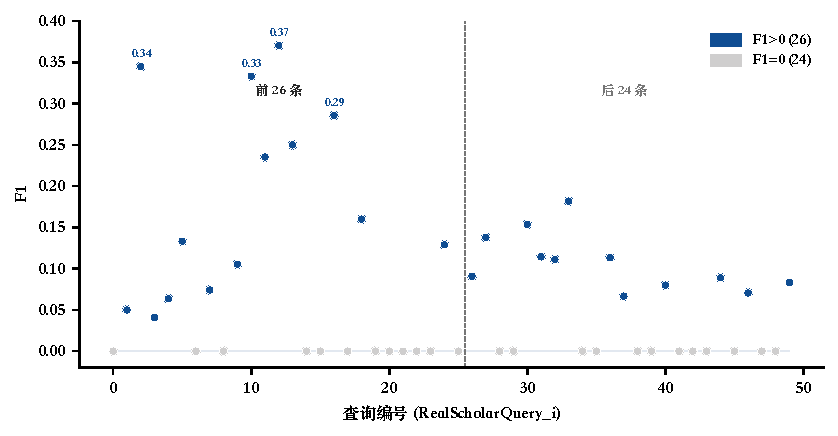
\includegraphics[width=0.92\textwidth]{fig3_per_query}
\caption{全链路在 50 条查询上的逐条 F1 分布（蓝色为 F1>0，灰色为 F1=0）。可见多数查询仍为零命中（召回覆盖不足是首要瓶颈），少数查询取得较高 F1（最高 0.37）。横轴为竞赛基准 PaSa RealScholarQuery 的 50 条真实复杂科研查询编号。}
\label{fig:perquery}
\end{figure}

\noindent\textbf{评测结论与失败归因}：全链路在 50 条查询上平均 F1 达 0.0774，约为词法基线的 8.2 倍，但仍有 24 条查询 F1=0，\textbf{召回仍是第一瓶颈}。对 22 条已覆盖查询中的 184 篇真值论文逐篇归因：162 篇（88.0\%）因词面与查询零重叠而\textbf{完全未进入候选池}，13 篇（7.1\%）在词法粗筛阶段被\textbf{挤出}，9 篇（4.9\%）在精排阶段被\textbf{降级}，\textbf{无任何假召回}。这一结论与 PaSa 论文"先解决召回覆盖、再优化排序"的判断高度一致，也验证了本系统失败归因框架的有效性。

进一步归类上述失败去向：其一，查询中的关键实体（方法名、数据集名、系统名）在目标论文标题中以别名或缩写形式出现，词面零重叠，构成\textbf{未召回}（88\%）的主体；其二，查询描述的科研任务过于宽泛，子查询难以覆盖真值论文所在的具体子方向；其三，真值论文发表于较冷门会议或非英语文献，单一数据源元数据收录不全。针对第一类，\textbf{联想词专名召回}（独立真值论文召回由基线 22 提升至 25）与\textbf{多源召回}（Semantic Scholar 在 OpenAlex 之上额外新增 13 篇真值论文，+7.1\%）已显著改善；针对第二类，需要更精细的子查询生成策略；针对第三类，可通过扩大召回源覆盖加以缓解。这一逐级归因的方法论，使后续优化始终有据可依，避免盲目调参。

\begin{table}[H]
\centering
\caption{失败去向归因（22 条已覆盖查询、184 篇真值论文；真值论文即基准中每条查询对应的人工标注正确论文）}
\label{tab:attribution}
\small
\begin{tabular}{@{}lccc@{}}
\toprule
\textbf{失败类别} & \textbf{篇数} & \textbf{占比} & \textbf{发生阶段} \\
\midrule
未召回（词面零重叠） & 162 & 88.0\% & 检索覆盖 \\
词法粗筛挤出 & 13 & 7.1\% & 词法过滤 \\
精排降级 & 9 & 4.9\% & 综合排序 \\
\midrule
合计（无假召回） & 184 & 100\% & --- \\
\bottomrule
\end{tabular}
\end{table}

\begin{figure}[H]
\centering
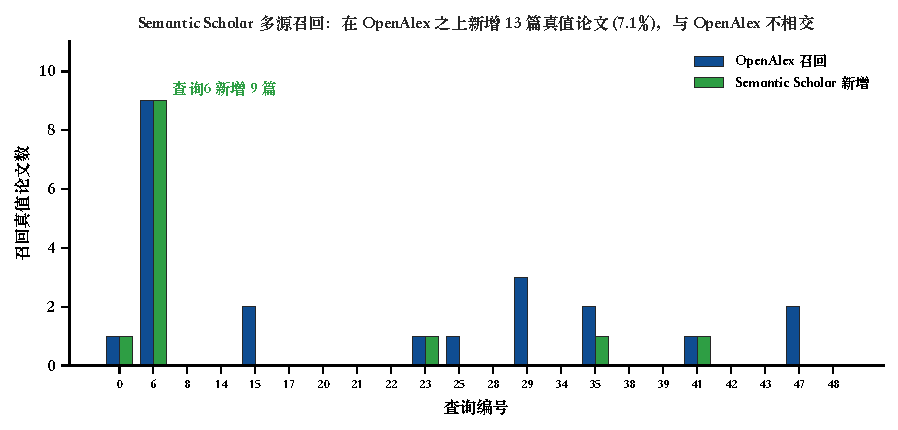
\includegraphics[width=0.92\textwidth]{fig5_direction1}
\caption{Semantic Scholar 多源召回增益（逐查询对照）。OpenAlex 单独召回 22 篇真值论文，叠加 Semantic Scholar 后新增 13 篇（+7.1\%）且与 OpenAlex 结果不相交，共 5 条查询受益。图中蓝色为各查询的 OpenAlex 召回量、绿色为 Semantic Scholar 新增量，其中查询 6 新增 9 篇（其目标论文含大量专名、词面与查询零重叠）。Semantic Scholar（S2）为另一主流开放学术文献数据库与检索 API。}
\label{fig:multisource}
\end{figure}

\begin{table}[H]
\centering
\caption{精排器消融（冻结候选池、22 条查询，各精排器输出候选数量一致；均为确定性方法）}
\label{tab:reranker}
\small
\begin{tabular}{@{}llcc@{}}
\toprule
\textbf{精排策略} & \textbf{类型} & \textbf{模型规模} & \textbf{宏平均 F1} \\
\midrule
大语言模型综合精排（生产） & 生成式 & --- & 0.0664 \\
MiniLM 句向量打分器 & 轻量嵌入 & 22M & 0.0598 \\
BGE 精排器 & 嵌入精排 & 568M & 0.0588 \\
RRF 词频融合 & 无模型 & --- & 0.0241 \\
\bottomrule
\end{tabular}
\end{table}

\begin{figure}[H]
\centering
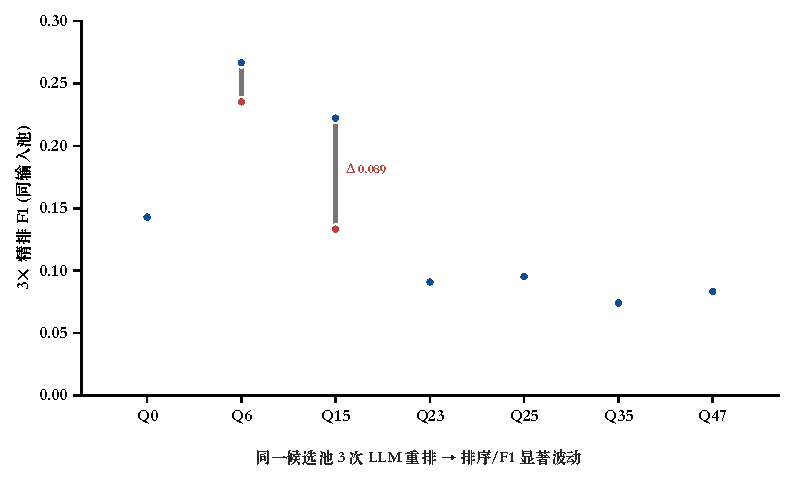
\includegraphics[width=0.8\textwidth]{fig7_stochasticity}
\caption{大语言模型精排的随机性（7 条高覆盖查询、同一候选池 3 次重复重排）。同一输入重复精排，F1 出现明显波动（最大差 0.089），说明生成式精排的排序结果非确定；这要求评测以多次运行或缓存回放保证可复现。红点与蓝点分别为 3 次重排的 F1 下界与上界。}
\label{fig:stochasticity}
\end{figure}

\begin{table}[H]
\centering
\caption{低收益扩展阶段的受控消融（FULL 与 NO\_CITATION 对比；历史冻结计划与响应缓存口径）}
\label{tab:budget}
\small
\begin{tabular}{@{}lccc@{}}
\toprule
\textbf{方案} & \textbf{平均 F1} & \textbf{逻辑 API 调用} & \textbf{结论} \\
\midrule
FULL（完整扩展链路） & 0.0528 & 511 & 引文/参考/元数据扩展占用 422 次调用、零新增命中 \\
NO\_CITATION（关闭低收益扩展） & 0.0618 & 87 & 成本下降约 83\%，F1 反而提升 \\
\bottomrule
\end{tabular}
\end{table}

\subsection{官方冻结评测与运行效率}
\label{sec:frozeneval}

在 50 条全量评测之外，项目依据竞赛复现要求构建了\textbf{官方冻结评测集}：从 RealScholarQuery 测试集冻结 22 条复杂查询（184 篇 paper-level Gold，corpus version 为 pasa\_realscholar\_test\_b3b570411ce2399c），统一数据文件、查询集合与 corpus fingerprint，避免不同阶段因数据版本或计数口径变化造成误判。FAST 与 DEEP 均采用 final-output-based 口径（以最终用户可见结果中的 Gold 命中计算 P/R/F1），retrieval-stage Gold 另行记录、不与 final Gold 混用：

\begin{table}[H]
\centering
\caption{S1 官方冻结评测结果（22 条复杂查询，184 篇 Gold）}
\label{tab:frozen}
\small
\begin{tabular}{@{}lccccc@{}}
\toprule
\textbf{模式} & \textbf{Precision} & \textbf{Recall} & \textbf{F1} & \textbf{final unique Gold} & \textbf{状态} \\
\midrule
FAST & 0.0842 & 0.0924 & 0.0680 & 14 & 离线冻结评测通过 \\
DEEP & 0.0797 & 0.0940 & 0.0641 & 15 & 离线冻结评测通过 \\
\bottomrule
\end{tabular}
\end{table}

FAST 在冻结集上的平均 F1 高于 DEEP，因此最终将 FAST 设为默认竞赛模式；DEEP 能执行证据引导的二轮检索并发现第一轮未覆盖论文（Round-2 新增独立真值论文 2 篇，62 个 follow-up 查询均在预算内），故保留为复杂问题的可选深度检索能力。

在模型与检索接口余额恢复后，系统完成了\textbf{真实在线冒烟评测}（真实 OpenAlex HTTP 与真实 DeepSeek 调用，非缓存回放），并区分逻辑 API 调用与物理 HTTP 请求：

\begin{table}[H]
\centering
\caption{真实在线运行效率（在线冒烟，非回放）}
\label{tab:online}
\small
\begin{tabular}{@{}lcccccl@{}}
\toprule
\textbf{模式} & \textbf{OpenAlex 调用/查询} & \textbf{LLM 调用/查询} & \textbf{Token/查询} & \textbf{平均时延 (ms)} & \textbf{P90 时延 (ms)} & \textbf{说明} \\
\midrule
FAST 在线 & 10.8 & 8.8 & 18,211 & 58,239 & $\approx$62,574 & 5/5 成功，标题完整率 100\% \\
DEEP 在线 & 12.5 & 11.0 & 24,124 & $\approx$79,202 & --- & 2/5 成功，部分受 OpenAlex 429 限流，仅参考 \\
\bottomrule
\end{tabular}
\end{table}

真实在线时延的主要来源是学术接口的物理往返与并发上限，而非算法逻辑本身；相比离线回放（frozen 产物物理 HTTP 调用为 0），在线时延反映真实部署成本。DEEP 在线冒烟受 OpenAlex 日配额限流影响仅 2/5 查询完整成功，其数字仅作参考、不作为正式效率结论，可在配额恢复后重跑补全。

\subsection{实施计划与团队分工}
\label{sec:schedule}

\begin{table}[H]
\centering
\caption{实施计划（已执行的阶段以$\bigstar$标记）}
\label{tab:schedule}
\small
\begin{tabular}{@{}llp{7cm}@{}}
\toprule
\textbf{阶段} & \textbf{时间} & \textbf{主要任务} \\
\midrule
S0 基线与评测（$\bigstar$） & 8/20--8/21 & 建仓、B0 基线、核心 Schema、评测框架、20 条挑战查询 \\
S1 查询理解（$\bigstar$） & 8/20--8/24 & Parser/Planner、子查询分解、联想词召回、B1 评测 \\
S2 引文扩展（$\bigstar$） & 8/21--8/24 & S2 / OpenCitations 双源引文、B2 评测、50 条全量 \\
S3 精排与全链路（$\bigstar$） & 8/22--8/24 & LLM 精排、FULL 全链路、早停决策、PaSa 全量评测 \\
S4 前端与归纳（$\bigstar$） & 8/22 & Web Demo、结构化归纳、引文关系图、轻量数据库 \\
S5 比赛冻结 & 8/25--9/9 & 冻结评测集、对齐 gold、FULL 冻结验证、复现包 \\
S6 答辩准备 & 9/9--9/11 & 材料整理、PPT、演示、专家分准备 \\
\bottomrule
\end{tabular}
\end{table}

\noindent\textbf{团队分工}（拟）：系统架构与核心算法（1 人）、评测与数据（1 人）、前后端与展示（1 人）、文档与答辩（1 人）。

\subsection{前端页面规划}
\label{sec:frontend}

为直观呈现系统的检索能力与结构化输出，项目规划了一个简洁的 Web 展示页面，包含四个核心区域：

\begin{itemize}
  \item \textbf{搜索入口}：提供查询输入框、模式选择（快速/深度）、归纳开关，支持输入后一键检索；
  \item \textbf{结果列表}：以卡片形式展示推荐论文，每张卡片包含标题、作者、年份、来源、相关度评分与推荐理由，点击可查看详情；
  \item \textbf{结构化归纳区}：展示查询摘要、论文分组与总体结论，帮助用户快速把握检索结果的整体结构；
  \item \textbf{引文关系图}：以可视化方式呈现核心论文与扩展论文之间的引用/被引关系，使用户直观理解检索的扩展路径。
\end{itemize}

该前端页面正在开发中，本节图 2 预留了页面截图的位置，页面完成验收后将替换为实际截图。前端采用轻量技术栈，通过 REST 接口调用后端服务，不引入额外的计算负担，保证演示环境的轻量化部署。

\subsection{风险分析与应对}
\label{sec:risk}

\begin{itemize}
  \item \textbf{API 配额风险}：OpenAlex 每日配额有限，可能影响大规模评测。应对：磁盘缓存复用、本地+服务器双 IP 并行、优先跑关键实验；
  \item \textbf{模型非确定性风险}：LLM 输出存在随机性，影响可复现评测。应对：计划缓存 + 冻结计划 + 温度设为 0，以缓存回放保证离线复现；
  \item \textbf{召回覆盖风险}：部分 gold 论文与查询词面零重叠。应对：联想词专名召回 + 引文图扩展双通道；
  \item \textbf{时间风险}：提交截止 9 月 11 日。应对：冻结时间窗前置到 9 月 9 日，为答辩预留缓冲。
\end{itemize}

\subsection{预期成果与交付物}
\label{sec:deliverables}

项目计划交付的成果物包括：

\begin{itemize}
  \item \textbf{可运行的检索系统}：完整实现的 eZScholar 后端服务（FastAPI 接口）与前端 Demo，支持 b0--full 多模式切换与结构化归纳展示；
  \item \textbf{冻结评测包}：冻结的 50 条 RealScholarQuery 评测集、gold 论文身份对齐表、评测脚本与复现说明，保证结果可复现、可审计；
  \item \textbf{结构化输出}：统一 JSON Schema 定义、前端渲染模板与字段完整性校验工具；
  \item \textbf{技术文档}：本提案、技术方案说明、评测报告、答辩演示材料；
  \item \textbf{证据链与执行轨迹}：SearchTrace 完整执行日志，可追溯每篇推荐论文的召回来源、扩展路径与精排理由。
\end{itemize}

这些交付物共同构成一个"可用、可复现、可解释、可答辩"的完整参赛方案，既满足比赛评测要求，也具备真实的科研应用价值。

% =========================================================
\section{参考资料}
\label{sec:references}

以下为项目技术与方案设计的权威支撑文献：

\begin{table}[H]
\centering
\caption{核心参考论文}
\label{tab:refs}
\small
\begin{tabular}{@{}lp{9.5cm}@{}}
\toprule
\textbf{编号} & \textbf{文献} \\
\midrule
\textbf{[1]} & He Y, et al. PaSa: An LLM Agent for Comprehensive Academic Paper Search. \emph{ACL 2025}. 提供 RealScholarQuery 基准与智能体式学术检索范式。 \\
\textbf{[2]} & Wang L, et al. Synergistic Interplay between Search and Large Language Models for Information Retrieval (InteR). \emph{ACL 2024}. 检索与 LLM 协同迭代框架。 \\
\textbf{[3]} & SPAR: Scholar Paper Retrieval with LLM-based Agents for Enhanced Academic Search. \emph{arXiv:2507.15245}. LLM 智能体学术检索增强。 \\
\textbf{[4]} & Huang J, et al. Knowledge-Aware Query Expansion with Large Language Models for Textual and Relational Retrieval (KAR). \emph{NAACL 2025}. 查询扩展与结构化关系利用。 \\
\textbf{[5]} & Yao H, et al. LLM-QE: Improving Query Expansion by Aligning Large Language Models with Ranking Preferences. 面向排序偏好的查询扩展。 \\
\textbf{[6]} & MILL: Mutual Verification with Large Language Models for Zero-Shot Query Expansion. \emph{arXiv:2310.19056}. 零样本查询扩展互验。 \\
\textbf{[7]} & SciRAG: Adaptive, Citation-Aware, and Outline-Guided Retrieval and Synthesis for Scientific Literature. \emph{arXiv:2511.14362}. 引文感知的学术检索与综合。 \\
\textbf{[8]} & Nogueira R, et al. Navigation-based candidate expansion and pretrained language models for citation recommendation. \emph{Scientometrics} 125(3), 2020. 引文图导航候选扩展 + 预训练模型重排。 \\
\textbf{[9]} & OpenAlex 项目文档与 API 文档. \emph{openalex.org}. 2.4 亿+ 学术成果开放元数据目录，CC-0 许可。 \\
\textbf{[10]} & Towards Optimizing a Retrieval Augmented Generation using Large Language Model on Academic Data. \emph{arXiv:2411.08438}. 学术领域 RAG 优化。 \\
\bottomrule
\end{tabular}
\end{table}

\noindent 上述文献为项目设计提供了直接依据：

\begin{itemize}
  \item 基准选择与评测口径：\cite{pasa2025} 的 RealScholarQuery；
  \item 查询理解与子查询分解：\cite{intr2024} 的检索--LLM 协同、\cite{kar2025} 的查询扩展；
  \item 引文扩展与候选放大：\cite{nogueira2020} 的引文图导航扩展、\cite{scirrag2025} 的引文感知检索；
  \item 精排与质量门禁：\cite{llmqe2024}、\cite{mill2024} 的 LLM 排序偏好与互验；
  \item 工程基础设施：OpenAlex 开放学术数据 \cite{openalex} 与免 Key API 生态。
\end{itemize}

\begin{thebibliography}{99}
\bibitem{pasa2025} Y.~He, H.~Jin, C.~Wu, H.~Lu, et al. PaSa: An LLM Agent for Comprehensive Academic Paper Search. In \emph{Proceedings of ACL 2025}, 2025.
\bibitem{intr2024} L.~Wang, et al. Synergistic Interplay between Search and Large Language Models for Information Retrieval. In \emph{Proceedings of ACL 2024}, 2024.
\bibitem{spar2025} SPAR: Scholar Paper Retrieval with LLM-based Agents for Enhanced Academic Search. \emph{arXiv:2507.15245}, 2025.
\bibitem{kar2025} J.~Huang, et al. Knowledge-Aware Query Expansion with Large Language Models for Textual and Relational Retrieval. In \emph{Proceedings of NAACL 2025}, 2025.
\bibitem{llmqe2024} H.~Yao, et al. LLM-QE: Improving Query Expansion by Aligning Large Language Models with Ranking Preferences. 2024.
\bibitem{mill2024} MILL: Mutual Verification with Large Language Models for Zero-Shot Query Expansion. \emph{arXiv:2310.19056}, 2024.
\bibitem{scirrag2025} SciRAG: Adaptive, Citation-Aware, and Outline-Guided Retrieval and Synthesis for Scientific Literature. \emph{arXiv:2511.14362}, 2025.
\bibitem{nogueira2020} R.~Nogueira, et al. Navigation-based candidate expansion and pretrained language models for citation recommendation. \emph{Scientometrics}, 125(3):2491--2513, 2020.
\bibitem{openalex} OurResearch. OpenAlex: A free, fully open catalog of the global research system. \url{https://openalex.org}, 2025.
\bibitem{ragacademic2024} Towards Optimizing a Retrieval Augmented Generation using Large Language Model on Academic Data. \emph{arXiv:2411.08438}, 2024.
\end{thebibliography}

\end{document}
